\chapter{2023/12/25}\label{20231225}

\section{Relationships between events in Minkowski spacetime
闵可夫斯基时空中的事件关系}\label{relationships-between-events-in-minkowski-spacetime-ux95f5ux53efux592bux65afux57faux65f6ux7a7aux4e2dux7684ux4e8bux4ef6ux5173ux7cfb}

Suppose in Minkowski spacetime, we have 2 events, for example,
\((ct_1, x_1, y_1, z_1)\) and \((ct_2, x_2, y_2, z_2)\). Then, the
spacetime interval (时空间隔) between the two events is
\[\Delta s^2 = (c \Delta t)^2 - \Delta x^2 - \Delta y^2 - \Delta z^2 = c^2 \Delta t^2 - \Delta \boldsymbol{r}^2,\]
where \(\Delta \boldsymbol{r}\) is the three-dimensional spatial
distance between the events, the time interval is \(c\Delta t\) and the
three spatial intervals are \(\Delta x\), \(\Delta y\), \(\Delta z\).

In that case, comparing \(\Delta s^2\) with \(0\) seems to be comparing
the distance light travels between the occurrence of the events with
their spatial separation. We now have the following definitions:

\begin{itemize}
\tightlist{}
\item
  If \(\Delta s^2 > 0\), or
  \(c^2 \Delta t^2 > \Delta \boldsymbol{r}^2\), the spatial separation
  is less than the distance light travels and the interval is called
  \textbf{timelike}.
\item
  If \(\Delta s^2 = 0\), or
  \(c^2 \Delta t^2 = \Delta \boldsymbol{r}^2\), the spatial separation
  is equal to the distance light travels and the interval is called
  \textbf{lightlike}.
\item
  If \(\Delta s^2 < 0\), or
  \(c^2 \Delta t^2 < \Delta \boldsymbol{r}^2\), the spatial separation
  is greater than the distance light travels and the interval is called
  \textbf{spacelike}.
\end{itemize}

Fig 29.1 is an illustration of the timelike, spacelike, and lightlike
regions in Minkowski spacetime. In the illustration, the \(z\)-axis is
eliminated for the convenience of drawing.

\begin{center}
    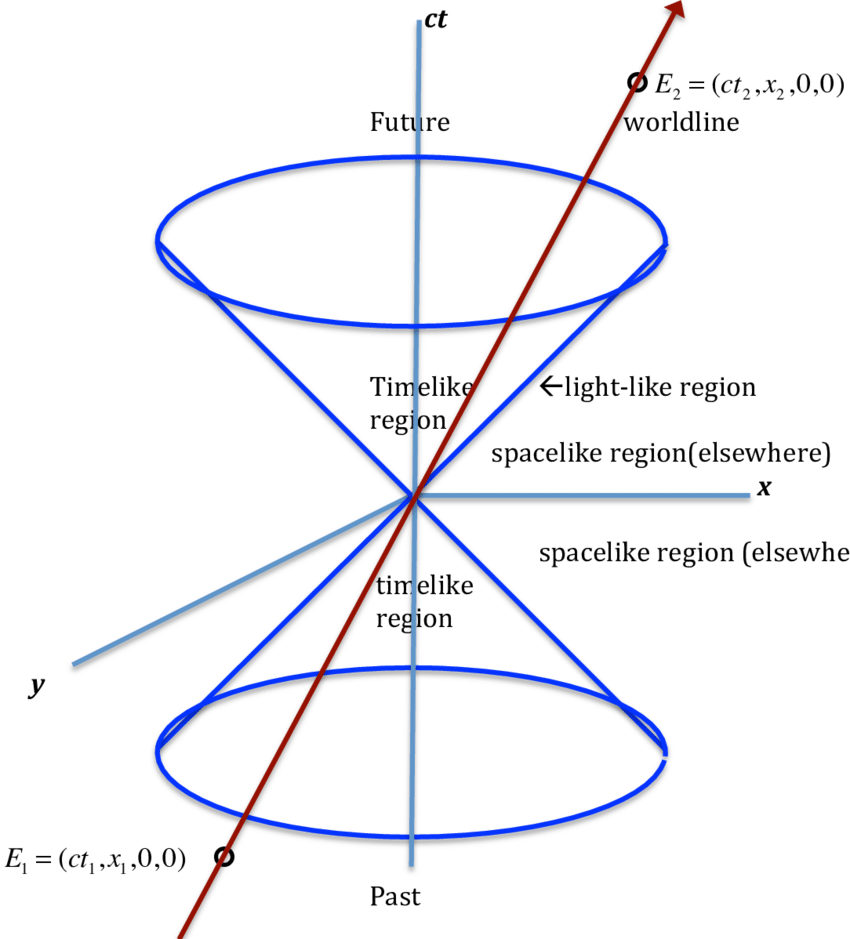
\includegraphics[height=320pt]{assets/Minkowski_spacetime.png}
    \captionof{figure}{Minkowski spacetime and relationships between events}
\end{center}

\emph{相对论的建立中,洛伦兹、庞加莱、闵可夫斯基等人都有杰出贡献,但最终认为爱因斯坦才是相对论的代表性人物,因为只有他形成了相对论中全链条的理论体系。}

\section{Further into relativity
相对论的进一步探讨}\label{further-into-relativity-ux76f8ux5bf9ux8bbaux7684ux8fdbux4e00ux6b65ux63a2ux8ba8}

\subsection*{(1) Postulates in special relativity
狭义相对论的公设}\label{postulates-in-special-relativity-ux72edux4e49ux76f8ux5bf9ux8bbaux7684ux516cux8bbe}

An \textbf{axiom (公理)} or \textbf{postulate (公设)} is a statement
that is taken to be true, to serve as a premise or starting point for
further reasoning and arguments. The difference between these two is
that axioms are statements taken to be true in \textbf{all subjects},
while postulates are statements taken to be true in \textbf{only a
particular subject}.

The two postulates in Einstein's special relativity are:

\begin{enumerate}
\def\labelenumi{\arabic{enumi}.}
\tightlist{}
\item
  The laws of physics have the same form in all inertial reference
  frames.
\item
  Light propagates through empty space with a definite speed \(c\)
  independent of the speed of the observer (or source).
\end{enumerate}

Last time, we talked about length contraction, which states that
\[L = L_0 \sqrt{1 - \frac{v^2}{c^2}}.\]

\begin{quote}
作业:贝尔飞船佯谬是什么?
\end{quote}

Max Born (波恩) put up with the problem of \textbf{Born rigidity}: if
the length of a rigid body would contract at high speeds, why is it a
rigid body?

There is strain (应变) as its definition
\[\varepsilon \overset{\text{def}}{=\!=} \frac{L - L_0}{L_0} = \sqrt{1 - \frac{v^2}{c^2}} - 1 \overset{v \ll c}{=\!=\!=} - \frac{v^2}{2 c^2},\]
and stress (应力) is \[\sigma = \varepsilon E = - E \frac{v^2}{2 c^2},\]
where \(E\) is the Young's modulus of the material.

\emph{从这里可以看出,这里应该是有力的,那么这到底是不是刚体?赵爹说,这是个科学哲学问题,下节课找两个同学辩论一下。}

\subsection*{(2) Time dilation
时间膨胀}\label{time-dilation-ux65f6ux95f4ux81a8ux80c0}

We suppose that there are 2 frames of reference \(S\) and \(S'\), and
\(S'\) is moving at a velocity \(\boldsymbol{v}\) relative to \(S\).

Consider 2 events at the same location in \(S\) happening at
\((t_1, x_1)\) and \((t_2, x_2)\), where \(x_1 = x_2\).

According to the Lorentz transformations, we have
\[t' = \gamma \left( t - \frac{vx}{c^2} \right),\] and with these two
events we get
\[t_2' - t_1' = \gamma \left[ t_2 - t_1 - \frac{v(x_2 - x_1)}{c^2} \right] = \gamma (t_2 - t_1).\]

Here \(\Delta \tau = t_2 - t_1\) is called \textbf{proper time
(固有时)}, and it means the time lapse between the two events in a frame
of reference (stationary frame) in which the two events happen at the
same location. The time measured in a frame of reference which has a
velocity relative to the stationary frame is greater than the proper
time. Thus the duration of the clock cycle of a moving clock is found to
be increased: it is measured to be ``running slow'', and that's where
the name ``time dilation'' comes from.

\section{Symplectic matrices
辛矩阵}\label{symplectic-matrices-ux8f9bux77e9ux9635}

\subsection*{(1) Comparing different formulations of classical
mechanics
对比经典力学的不同表述}\label{comparing-different-formulations-of-classical-mechanics-ux5bf9ux6bd4ux7ecfux5178ux529bux5b66ux7684ux4e0dux540cux8868ux8ff0}

\begin{center}
    \begin{tabular}{|c|c|c|}
        \hline
        \textbf{Formulations} & \textbf{Physical contrast} & \textbf{Mathematical contrast} \\
        \hline
        \rule{0pt}{20pt}
        \textbf{Newtonian mechanics} & $\displaystyle \boldsymbol{F} = \frac{\mathrm{d}p}{\mathrm{d}t}$ & Euclidean geometry \\
        \hline
        \rule{0pt}{20pt}
        \textbf{Lagrangian mechanics} & $\displaystyle \frac{\partial L}{\partial q_j} - \frac{\mathrm{d}}{\mathrm{d}t} \frac{\partial L}{\partial \dot{q}_j} = 0$ & Riemann geometry \\
        \hline
        \rule{0pt}{35pt}
        \textbf{Hamiltonian mechanics} & $\displaystyle \left\{ \begin{aligned} \frac{\partial H}{\partial q_j} &= -\dot{p}_j, \\ \frac{\partial H}{\partial p_j} &= \dot{q}_j \end{aligned} \right.$ & Symplectic geometry \\
        \hline
        \textbf{Equivalency} & Physically equivalent & Mathematically not equivalent \\
        & (物理上等价) & (数学上不等价) \\
        \hline
    \end{tabular}
    \captionof{table}{Comparing different formulations of classical mechanics}
\end{center}

\subsection*{(2) Symplectic matrix
辛矩阵}\label{symplectic-matrix-ux8f9bux77e9ux9635}

Hermann Weyl developed the theory of \textbf{symplectic matrices
(辛矩阵)}, which write the Hamiltonian canonical equations (as shown in
the table above) in matrix form (one-degree): \[\begin{pmatrix}
    \dot{q} \\
    \dot{p}
\end{pmatrix} = \begin{pmatrix}
    0 & 1 \\
    -1 & 0
\end{pmatrix} \begin{pmatrix}
    \displaystyle \frac{\partial H}{\partial q} \\[1.5ex]
    \displaystyle \frac{\partial H}{\partial p}
\end{pmatrix}.\]

If there are \(n\) generalized coordinates, the form of the symplectic
matrix would be \begin{align*}
    \begin{pmatrix}
        \dot{q}_1 \\
        \dot{q}_2 \\
        \vdots \\
        \dot{q}_n \\
        \dot{p}_1 \\
        \dot{p}_2 \\
        \vdots \\
        \dot{p}_n
    \end{pmatrix} & = \begin{pmatrix}
        0 & 0 & \cdots & 0 & 1 & 0 & \cdots & 0 \\
        0 & 0 & \cdots & 0 & 0 & 1 & \cdots & 0 \\
        \vdots & \vdots & \ddots & \vdots & \vdots & \vdots & \ddots & \vdots \\
        0 & 0 & \cdots & 0 & 0 & 0 & \cdots & 1 \\
        -1 & 0 & \cdots & 0 & 0 & 0 & \cdots & 0 \\
        0 & -1 & \cdots & 0 & 0 & 0 & \cdots & 0 \\
        \vdots & \vdots & \ddots & \vdots & \vdots & \vdots & \ddots & \vdots \\
        0 & 0 & \cdots & -1 & 0 & 0 & \cdots & 0 \\
    \end{pmatrix}_{2n \times 2n} \begin{pmatrix}
        \partial H / \partial q_1 \\
        \partial H / \partial q_2 \\
        \vdots \\
        \partial H / \partial q_n \\
        \partial H / \partial p_1 \\
        \partial H / \partial p_2 \\
        \vdots \\
        \partial H / \partial p_n \\
    \end{pmatrix}  \\
    & = \begin{pmatrix}
        \mathbf{0}_n & \mathbf{I}_n \\
        - \mathbf{I}_n & \mathbf{0}_n
    \end{pmatrix} \begin{pmatrix}
        \partial H / \partial q_1 \\
        \partial H / \partial q_2 \\
        \vdots \\
        \partial H / \partial q_n \\
        \partial H / \partial p_1 \\
        \partial H / \partial p_2 \\
        \vdots \\
        \partial H / \partial p_n \\
    \end{pmatrix}.  \\
\end{align*}

Here, $\begin{pmatrix}
        \mathbf{0}_n & \mathbf{I}_n \\
        - \mathbf{I}_n & \mathbf{0}_n
    \end{pmatrix}$ is the symplectic matrix.

\section{Relativistic energy-time relationships
能量-动量关系}\label{relativistic-energy-time-relationships-ux80fdux91cf-ux52a8ux91cfux5173ux7cfb}

\subsection*{(1) Hamiltonian under relativistic conditions
相对论条件下的哈密顿量}\label{hamiltonian-under-relativistic-conditions-ux76f8ux5bf9ux8bbaux6761ux4ef6ux4e0bux7684ux54c8ux5bc6ux987fux91cf}

From last class, we know that
\[L = T - V = - mc^2 \sqrt{1 - \frac{\dot{q}^2}{c^2}} - V.\]

Thus, using Legendre transformation, we get \begin{align*}
    H & = p \dot{q} - L \\
    & = \frac{m \dot{q}}{\sqrt{1 - \dot{q}^2 / c^2}} \dot{q} - \left( - mc^2 \sqrt{1 - \frac{\dot{q}^2}{c^2}} - V \right) \\
    & = \frac{m \dot{q}^2}{\sqrt{1 - \dot{q}^2 / c^2}} + \frac{mc^2 \left( 1 - \dfrac{\dot{q}^2}{c^2} \right)}{\sqrt{1 - \dot{q}^2 / c^2}} + V \\
    & = \frac{m c^2}{\sqrt{1 - \dot{q}^2 / c^2}} + V = \gamma mc^2 + V.
\end{align*}

Let the potential energy \(V\) be \(0\), and we get the form of the
Hamiltonian under relativistic conditions: \[H = \gamma mc^2.\]

\subsection*{(2) Dirac energy-motion relation
狄拉克动量-能量关系}\label{dirac-energy-motion-relation-ux72c4ux62c9ux514bux52a8ux91cf-ux80fdux91cfux5173ux7cfb}

If the mass of a particle when stationary (invariant/proper mass,
固有质量) is \(m_0\), then under relativistic conditions its mass would
become \(m = \gamma m_0\). Thus, the total energy of the particle is
\begin{align*}
    E^2 & = m^2 c^4 = \gamma^2 m_0^2 c^4 = \frac{m_0^2 c^4}{1 - \dfrac{v^2}{c^2}} \\
    & = \frac{\displaystyle m_0^2 c^4 \left( 1 - \frac{v^2}{c^2} + \frac{v^2}{c^2} \right)}{1 - \dfrac{v^2}{c^2}} = m_0^2 c^4 + \frac{m_0^2 c^2 v^2}{1 - \dfrac{v^2}{c^2}} \\
    & = m_0^2 c^4 + \left( \frac{m_0 v}{\sqrt{1 - v^2 / c^2}} \right)^2 c^2 = m_0^2 c^4 + p^2 c^2,
\end{align*} which is the energy-momentum relation.

\subsection*{(3) Klein-Gordon equation
克莱因-戈尔登方程}\label{klein-gordon-equation-ux514bux83b1ux56e0-ux6208ux5c14ux767bux65b9ux7a0b}

We already know the momentum and energy operators in quantum mechanics:
\[\hat{\boldsymbol{p}} = - \mathrm{i} \hbar \nabla \quad \text{and} \quad \hat{E} = \mathrm{i} \hbar \frac{\partial}{\partial t}.\]

Operatorize the energy-momentum relation, and we get
\[E^2 \psi = (m_0^2 c^4 + p^2 c^2) \psi\]
\[\hat{E}^2 \psi = (m_0^2 c^4 + \hat{\boldsymbol{p}} \cdot \hat{\boldsymbol{p}} c^2) \psi\]
\[\left( \mathrm{i} \hbar \frac{\partial}{\partial t} \right)^2 \psi = \left[ \left( {i} \hbar \nabla \cdot {i} \hbar \nabla \right) c^2 + m_0^2 c^4 \right] \psi\]
\[- \hbar^2 \frac{1}{c^2} \frac{\partial^2 \psi}{\partial t^2} = \left( - \hbar^2 \nabla^2 + m_0^2 c^2 \right) \psi\]
\[\left( \frac{1}{c^2} \frac{\partial^2 }{\partial t^2} - \nabla^2 \right) \psi + \left( \frac{m_0c}{\hbar} \right)^2 \psi = 0.\]

Substitute
\(\displaystyle \frac{1}{c^2} \frac{\partial^2 }{\partial t^2} - \nabla^2 = \Box\)
and \(\displaystyle \frac{m_0c}{\hbar} = \mu\) in, and we get
\[\left( \Box + \mu^2 \right) \psi = 0.\]

The Klein-Gordon equation can reflect relativistic effects
(能反映相对论效应), but the second-order derivative with respect to time
contained in it makes it unable to reflect quantum behavior
(反映量子行为).

\emph{薛定谔:这个方程里面有时间的二阶导、没有虚数单位
\({\mathrm{i}}\),我不喜欢,我不发表。}

\emph{克莱因、戈尔登:你嫌弃,我们喜欢啊!于是发表。}

\section[Classical mechanics VS. special
relativity 对比经典力学和狭义相对论]{Comparison between classical mechanics and special
relativity
经典力学和狭义相对论的对比}\label{comparison-between-classical-mechanics-and-special-relativity-ux7ecfux5178ux529bux5b66ux548cux72edux4e49ux76f8ux5bf9ux8bbaux7684ux5bf9ux6bd4}

Below, we compare classical mechanics and special relativity:

\begin{center}
    \begin{tabular}{|c|c|c|}
        \hline
        & Classical mechanics & Special relativity \\
        \hline
        Trait & Stays invariant under & Stays invariant under \\ & Galilean transformations & Lorentz transformations \\
        \hline
        Related Group & Galilean group& Poincaré group \\
        & 伽利略群 & 庞加莱群 \\
        \hline
        Dimension of Group & 10 & 10 \\
        群的维数 & & \\
        \hline
    \end{tabular}
    \captionof{table}{Comparison of Classical Mechanics and Special Relativity}
\end{center}

\paragraph{Poincaré group: 10 dimensions}
\begin{itemize}
\tightlist{}
    \item 4: translation through time or space, one per dimension (时空维度的平移)
    \item 6: Lorentz group:
    \begin{itemize}
\tightlist{}
        \item 3: reflection through a plane, the freedom in orientation of this plane (关于三个平面的反射)
        \item 3: a "boost" in any of the three spatial directions (三个方向的递升)
    \end{itemize}
\end{itemize}

\paragraph{Galilean group: 10 dimensions}
\begin{itemize}
\tightlist{}
    \item 3: translation with uniform velocity (平移变换)
    \item 4: spatial and time translation (时空仿射变换)
    \item 3: rotation (旋转变换)
\end{itemize}

\emph{12月6日的笔记中有更详细的伽利略群的说明。}
